\subsubsection{Role Based Access Control} \label{sec:sota-rbac}

\acrfull{rbac} is a method of controlling users' access in the system (physical or online access) in the enterprise. It uses policy neutral approach based on roles, where every employee has one or more roles assigned, which define the access levels to resources. 
%Mandatory Access Control (MAC)\footnote{\url{https://nvlpubs.nist.gov/nistpubs/SpecialPublications/NIST.SP.800-53r4.pdf}, accessed 21 May 2019} and Discretionary Access Control (DAC)\footnote{\url{https://nvlpubs.nist.gov/nistpubs/SpecialPublications/NIST.SP.800-53r4.pdf}, accessed 21 May 2019} can also be implemented within the system, even though it is different from them.
\acrshort{rbac} creates a structure, where firstly the list of privileges (actions, resources, access levels) is defined and assigned to roles. Each role contains a set of privileges and is part of a group where more roles are gathered. Each employee is then assigned one or more groups or directly a role which authorizes them to access certain resources. This allows more effective management of employees.~\cite{Sandhu1996Role-basedModels}

The biggest drawback of \acrshort{rbac} is the manual process of assigning roles and groups, based on request, and not automated. Therefore, when an employee changes a position within a company and new roles are assigned, the previous roles should be revoked. This may be forgotten or overlooked by the responsible personnel and the employee is gradualy granted access to more and more resources. Furthermore, it can take a long time before a new role is assigned. Audit of roles and employees’ assignment to them needs to be carried out on a regular basis.

% % TODO explanation + diagram
% \begin{figure}[ht]
%     \centering
%     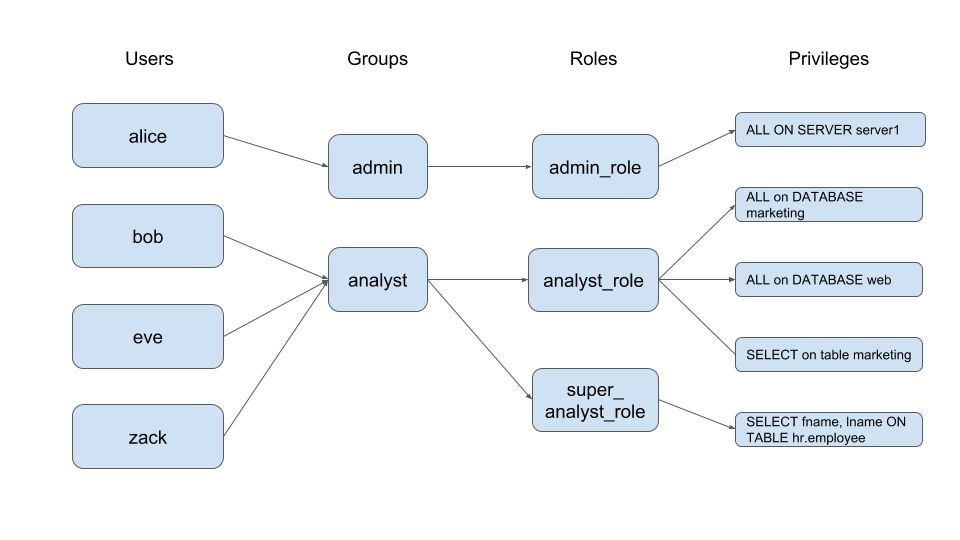
\includegraphics[width=.95\textwidth]{RBAC}
%     \caption{Explanation! + new diagram XYZ}
%     \label{fig:RBAC_diagram_sota}
% \end{figure}